\section{Results}

\subsection{Study Selection}

% PRISMA Diagram
\begin{figure*}[t]
\centering
\includegraphics[width=\textwidth]{figures/prisma_diagram.jpeg}
\caption{PRISMA flow diagram summarising the study selection process.}
\label{fig:prisma}
\end{figure*}

\noindent Details on the screening and selection process are demonstrated in Figure~\ref{fig:prisma}. Detail on independent inter-reviewer agreement and third author review can be found in Appendix~\ref{appendix:screening_results}. Significantly, 135 reports were excluded for failing to explicitly state whether the ingestion report was intentional. Another 91 were excluded for not reporting motivation. 

\subsection{Risk of Bias}
\input{sections/risk_of_bias_results.tex}

\input{tables/case_report_table.tex}

\subsection{Study Characteristics}
\input{sections/study_characteristics.tex}

\begin{figure}[htbp]
\centering
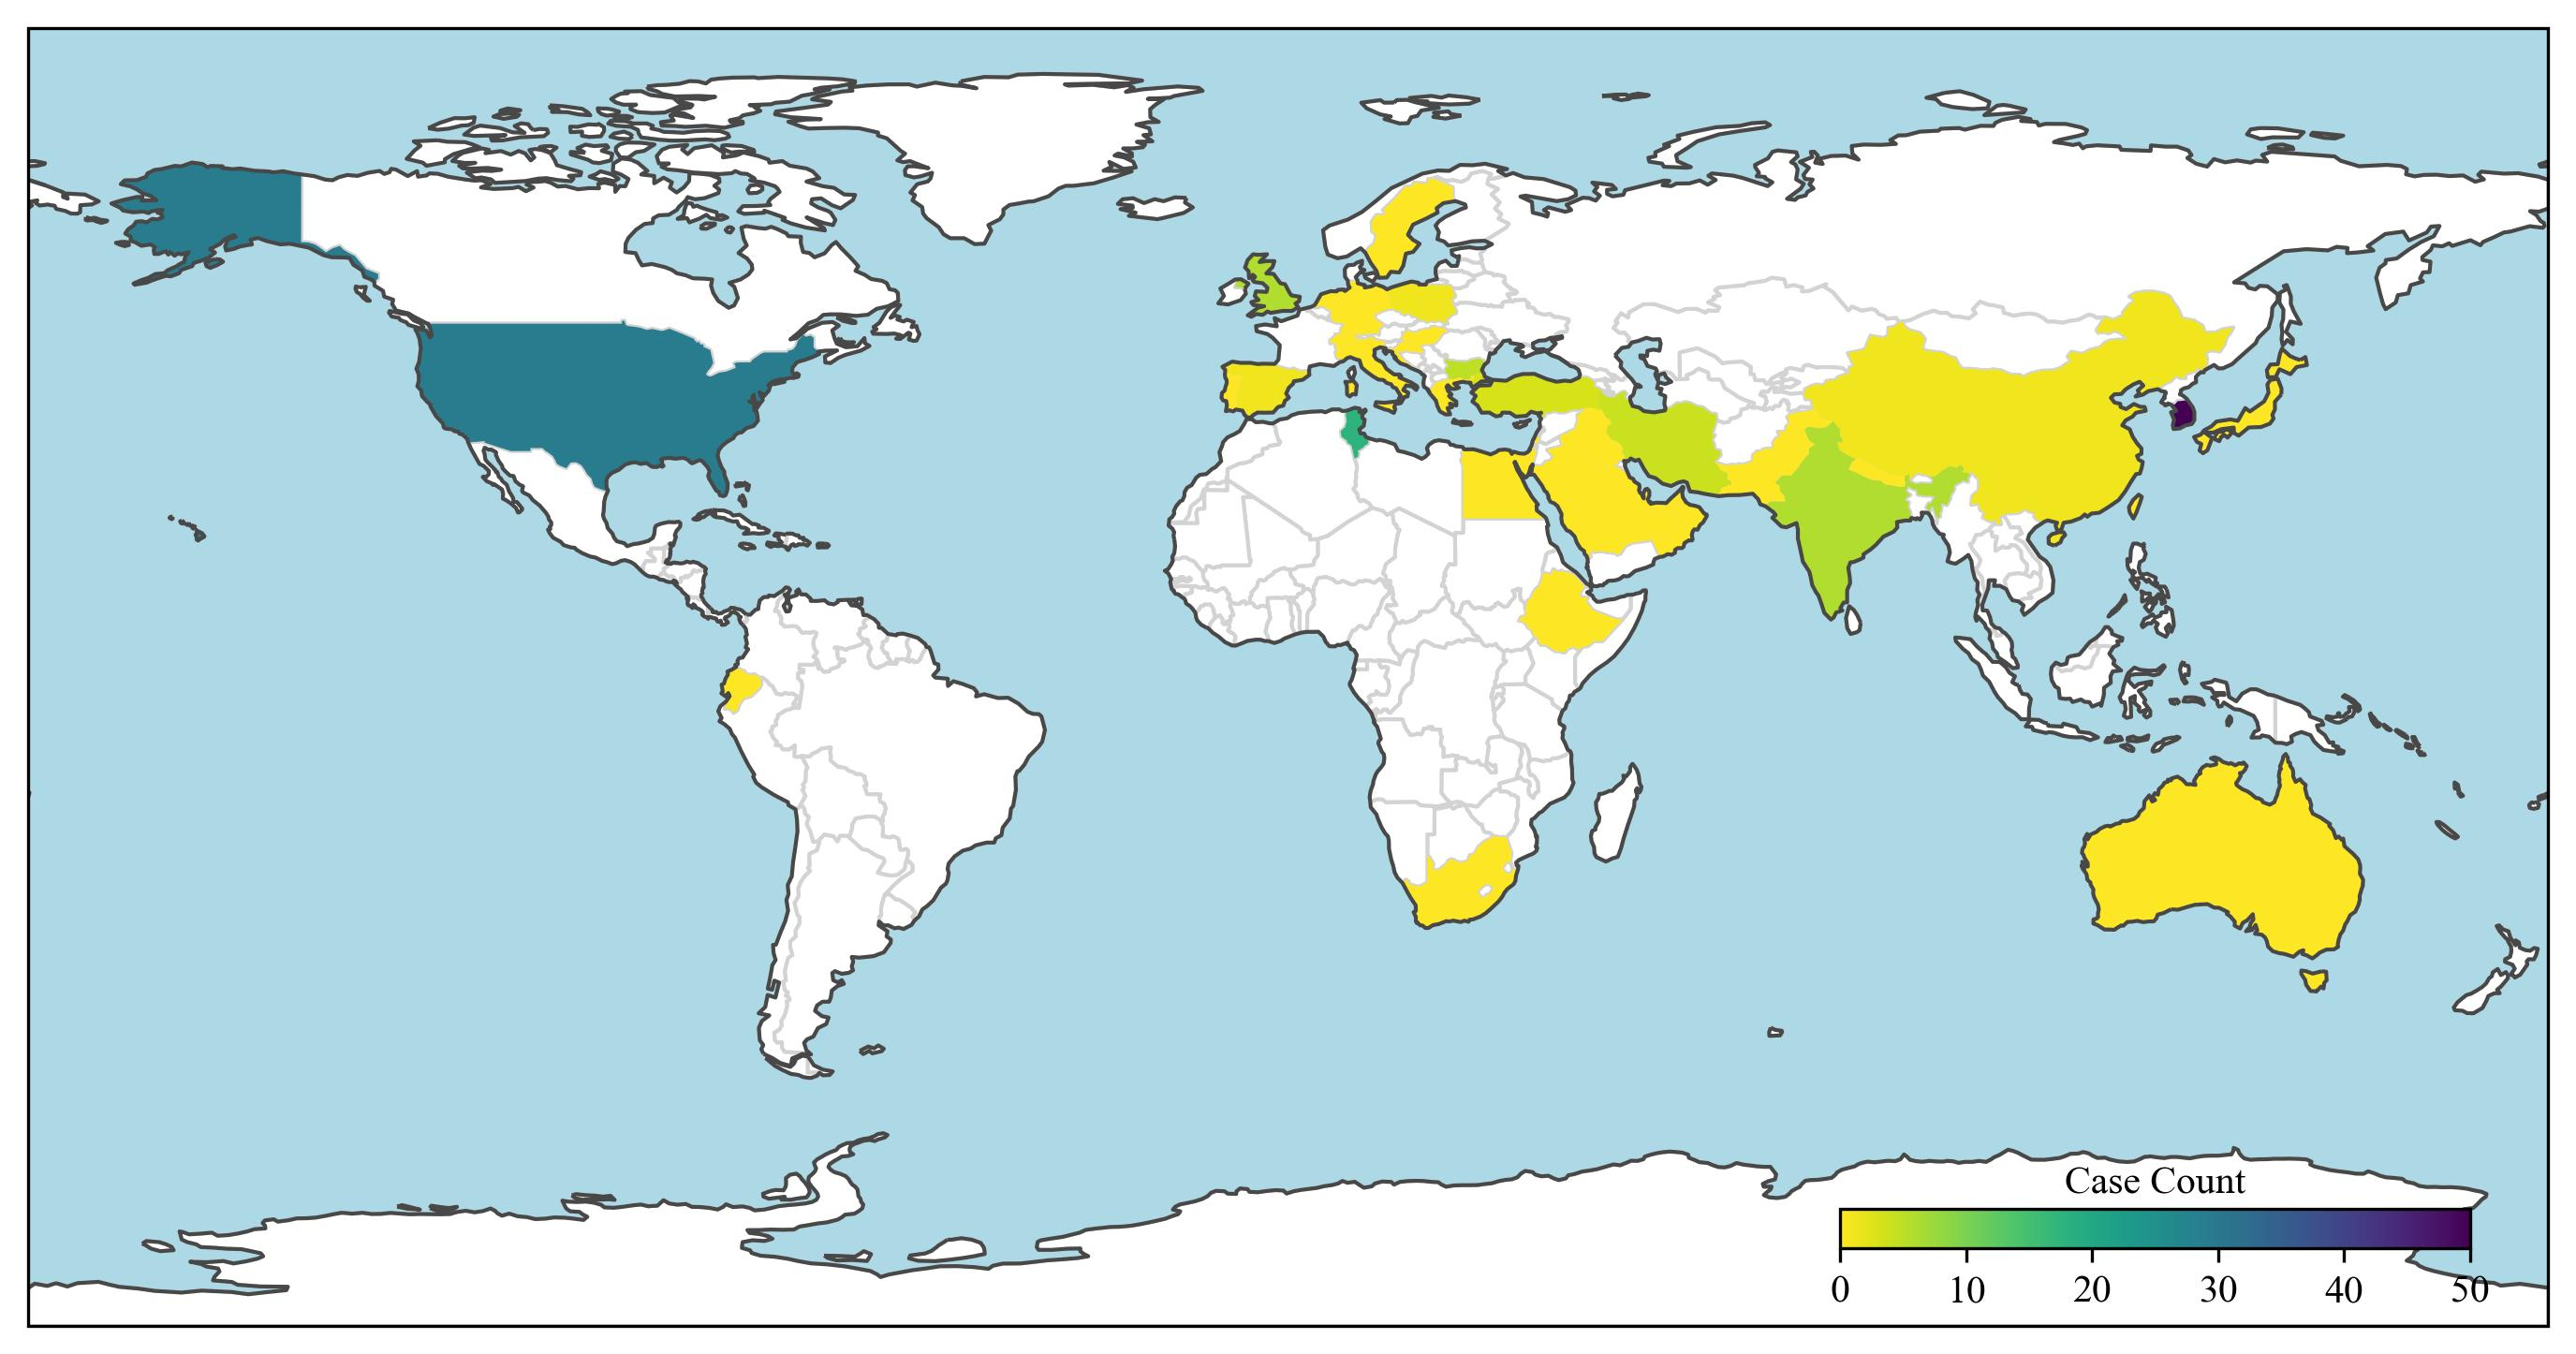
\includegraphics[width=\columnwidth]{figures/case_country_plot.jpeg}
\caption{Heat map of all cases per country.}
\label{fig:country_plot}
\end{figure}

\input{tables/country_table.tex}

\input{tables/case_series_table.tex}

\input{sections/synthesis.tex}

\input{sections/discussion.tex}

\begin{figure}[h]
\centering
 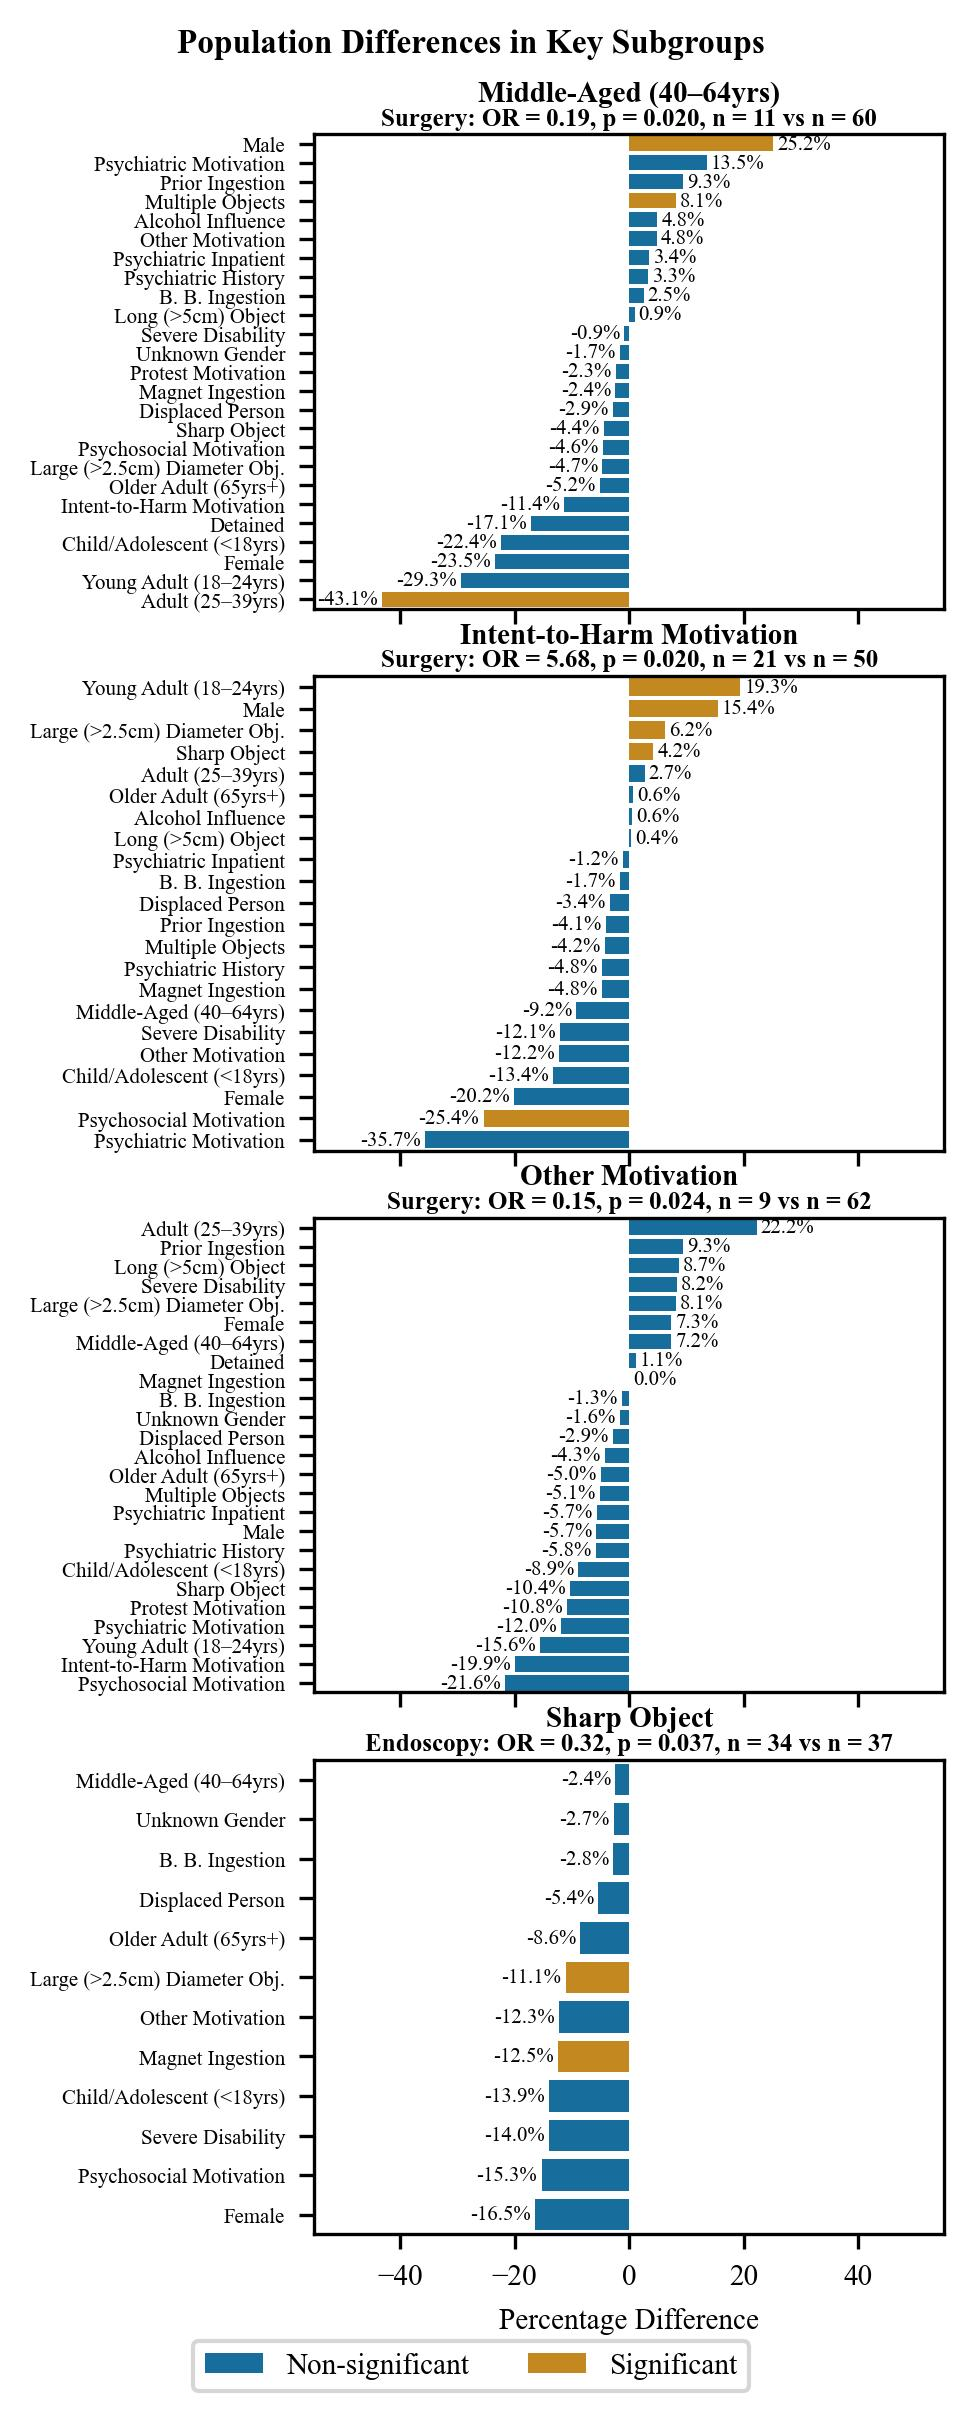
\includegraphics[width=\columnwidth, height=0.9\textheight, keepaspectratio]{figures/case_subgroup_analysis.jpeg}
\caption{Significant associated predictors from univariate analysis.}
\label{fig:case_subgroup_plot}
\end{figure}
